\subsection{要求分析}

\term{要求分析}とは、獲得された候補要求の意味、妥当性、矛盾、実現可能性、影響を調べる活動である。要求は、最初から完成形で出てくるとは限らない。多くの場合、曖昧、過剰、矛盾、不足、または解決策の断片として現れる。分析の目的は、それを真の要求へ近づけることである。

\subsubsection{要求の性質}

よい要求には、個々の要求として望ましい性質と、要求集合として望ましい性質がある。

\paragraph{個々の要求の望ましい性質}

\par\smallskip\noindent\refstepcounter{table}\label{tab:ch01-08}\textbf{表 \thetable: 第01章 ソフトウェア要求 表08}\par\smallskip
\begin{tabularx}{0.97\linewidth}{@{}p{.26\linewidth}X@{}}
\toprule
性質 & 説明 \\
\midrule
\term{一意に解釈できる} & 読む人によって意味が変わらない。 \\
\term{テスト可能である} & 満たしたかどうかを確認できる。必要なら数値で示す。 \\
\term{拘束力がある} & 顧客がそれに価値を認め、満たされないことを受け入れない。 \\
\term{原子的である} & 一つの要求が一つの判断だけを表す。 \\
\term{真のニーズを表す} & 単なる思いつきや特定解ではなく、実際の問題に基づく。 \\
\term{利害関係者の語彙を使う} & 利用者や業務専門家が理解できる言葉で書く。 \\
\term{関係者に受け入れられる} & 重要な利害関係者が納得できる。 \\
\bottomrule
\end{tabularx}

\paragraph{要求集合の望ましい性質}

\par\smallskip\noindent\refstepcounter{table}\label{tab:ch01-09}\textbf{表 \thetable: 第01章 ソフトウェア要求 表09}\par\smallskip
\begin{tabularx}{0.97\linewidth}{@{}p{.26\linewidth}X@{}}
\toprule
性質 & 説明 \\
\midrule
\term{完全性} & 通常ケースだけでなく、境界条件、例外条件、セキュリティ上の必要事項も扱う。 \\
\term{簡潔性} & 不要な記述や重複が少ない。 \\
\term{内部整合性} & 要求同士が矛盾しない。 \\
\term{外部整合性} & 契約、法令、標準、業務文書などの外部資料と矛盾しない。 \\
\term{実現可能性} & 費用、納期、人員、技術制約の範囲で実現できる。 \\
\bottomrule
\end{tabularx}

\MiniBox{5つのなぜ}{要求が解決策の形で出てきたときは、「なぜそれが必要なのか」を繰り返し問う。目的は、相手が本当に解決したい問題に到達することである。}

\subsubsection{サービス品質要求の経済性}

サービス品質制約は、単に「高ければよい」ものではない。たとえば、応答時間を極限まで短くする、稼働率を極限まで高くする、処理能力を極限まで大きくするには、費用が増える。したがって、要求は価値と費用の関係で考える必要がある。

\term{失敗点}は、それを下回るとシステムとして価値がほとんどなくなる水準である。\term{完全点}は、それを超えても利用者に追加価値がほとんど出ない水準である。現実的には、要求値はこの間で決まる。最もよい水準は、価値と費用の差が最大になる点である。

\begin{figure}[htbp]
\centering
\IfFileExists{assets/generated_figures/ch01/fig-ch01-07.png}{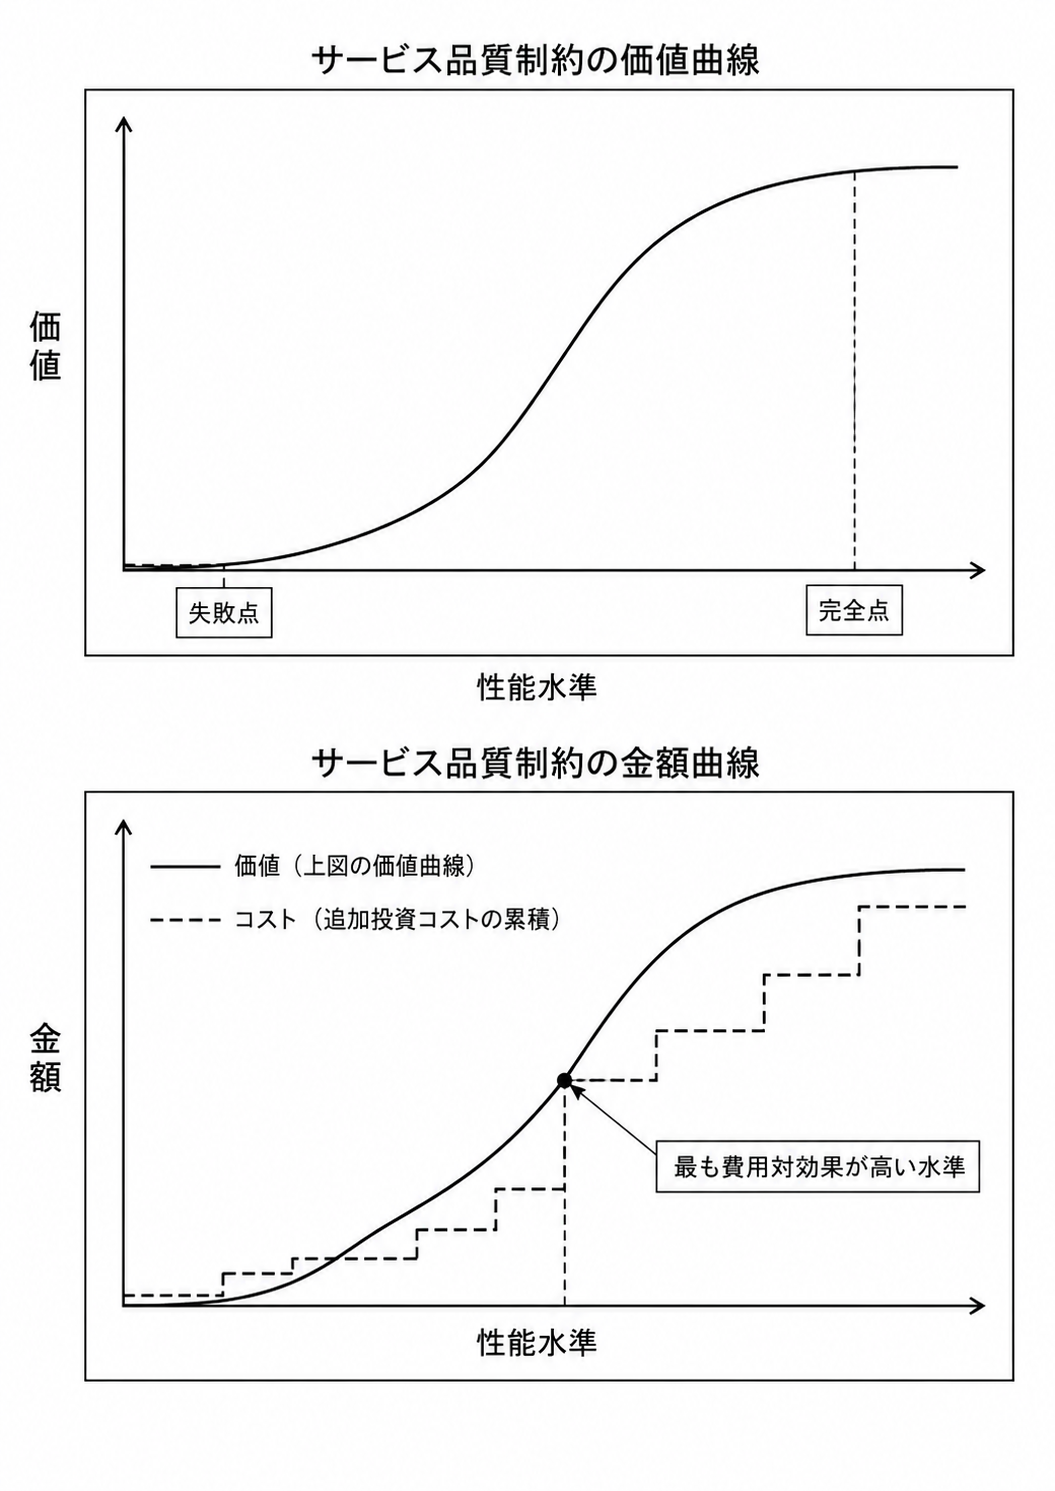
\includegraphics[width=0.96\linewidth]{assets/generated_figures/ch01/fig-ch01-07.png}}{\fbox{\parbox[c][48mm][c]{0.9\linewidth}{\centering 画像生成待ち\\サービス品質制約の価値・費用曲線}}}
\caption{サービス品質制約の価値・費用曲線}
\label{fig:ch01-07}
\end{figure}

サービス品質制約同士には、よい関係と悪い関係がある。たとえば、コードを単純にすると信頼性と変更容易性が同時に上がることがある。一方、実行速度を極端に高める最適化が、コードを複雑にして変更容易性を下げることもある。

\subsubsection{形式的分析}

\term{形式的分析}とは、数学的に意味が定義された言語やモデルを使って、要求を精密に表し、性質を検査する方法である。たとえば、デッドロックが起きないこと、特定の状態へ必ず到達すること、矛盾した状態が存在しないことなどを確認するために使われる。

形式的分析の利点は、曖昧さを減らせること、要求を論理的に推論できること、通常のレビューでは見落としやすい性質を確認できることである。一方で、記法を学ぶ負担があり、すべてのプロジェクトに適するわけではない。安全性や信頼性が非常に重要な領域で特に価値が高い。

\subsubsection{要求の衝突への対応}

利害関係者が多いほど、要求の衝突は起こりやすい。たとえば、利用者は高機能を求め、運用担当は単純で安定した運用を求め、経営側は費用や納期を抑えたいと考えることがある。

衝突への対応には、主に二つの方向がある。第一に、関係者間で交渉し、合意を形成することである。技術者が独断で決めると、責任や契約上の問題が残ることがある。第二に、\term{製品群開発}の考え方を使い、すべての利用者に共通する不変要求と、利用者や市場によって変わる可変要求を分けることである。

\MiniBox{例}{天気アプリで、ある利用者は摂氏表示を求め、別の利用者は華氏表示を求める。この場合、温度を表示することは共通要求であり、単位は可変要求である。}
